
\documentclass{beamer}
\mode<presentation>{\usetheme{Madrid}}
\usepackage{graphicx,amssymb,amsmath,tikz-cd,adjustbox}
\setbeamertemplate{navigation symbols}{}
%\setbeamertemplate{footline}[page number]{}

\DeclareMathOperator{\T}{T}
\DeclareMathOperator{\I}{I}
\DeclareMathOperator{\M}{M}
\DeclareMathOperator{\S}{S}
\DeclareMathOperator{\R}{R}
\DeclareMathOperator{\F}{F}
\DeclareMathOperator{\Aut}{Aut}
\DeclareMathOperator{\Fix}{Fix}
\DeclareMathOperator{\Aff}{Aff}
\DeclareMathOperator{\Ext}{Ext}
\DeclareMathOperator{\Toc}{Toc}

\title[Thesis Proposal]{GENERALIZED MULTIPLE ORDER-NUMBER FUNCTION ARRAYS}
\author{Luis F. Vieira Damiani}
\institute[UF]{University of Florida\\
\medskip
\textit{damiani@ufl.edu}}
\date{\today}

\begin{document}
\begin{frame}
\titlepage
\end{frame}


%------------------------------------------------------------------------
\begin{frame}
	\frametitle{Derivation}
	\begin{block}{Definition}
		\textbf{Derivation} is the process of extracting ordered segments from rows in order to generate new compositional materials. It dates back to the Second Viennese School.
	\end{block}
	\begin{block}{Motivation}
		\begin{itemize}
		\item The choice of a particular segment is an important compositional decision, as it establishes motivic material.
		\item It introduces complementary harmonic regions, one given by the segment, the other given by its set complement.
		\item It maintains motivic coherence under the chosen segment, while producing contrasting harmonic regions.
		\item It presents an opportunity for exploring syntax.
	\end{itemize}
	\end{block}
\end{frame}

%------------------------------------------------------------------------
\begin{frame}
	\frametitle{Derivation with the Retrograde}
	\begin{block}{Example}%\begin{example}
		Create a $2 \times 24$ array where the first row is $S$ followed by $\R(S)$, and the second row is initially undefined.
		\begin{equation*}
		\begin{adjustbox}{width=\textwidth}
			$\left[\begin{array}{cccccccccccc|cccccccccccc}
		10 & 2 & 3 & 0 & 5 & 7 & 4 & 6 & 9 & 8 & 1 & 11 & 11 & 1 & 8 & 9 & 6 & 4 & 7 & 5 & 0 & 3 & 2 & 10 \\
			. & . & . & . & . & . & . & . & . & . & . & . & . & . & . & . & . & . & . & . & . & . & . & .
			\end{array}\right]$
		\end{adjustbox}
		\end{equation*}
		Choose an arbitrary segment, and separate it from the the top row by placing in in the bottom row.
		\begin{equation*}
		\begin{adjustbox}{width=\textwidth}
			$\left[\begin{array}{cccccccccccc|cccccccccccc}
			. & 2 & 3 & . & . & . & 4 & 6 & 9 & 8 & 1 & 11 & . & . & . & . & . & . & 7 & 5 & 0 & . & . & 10 \\
			10 & . & . & 0 & 5 & 7 & . & . & . & . & . & . & 11 & 1 & 8 & 9 & 6 & 4 & . & . & . & 3 & 2 & .
			\end{array}\right]$
		\end{adjustbox}
		\end{equation*}
		The row $V = \{ 2, 3, 4, 6, 9, 8, 1, 11, 7, 5, 0, 10 \}$ is a row derived from $S$, where the ordered segment $\{ 10, 0, 5, 7 \}$ in $S$ is preserved by $\R(V)$.
	\end{block}%\end{example}
\end{frame}

%------------------------------------------------------------------------
\begin{frame}
	\frametitle{Producing Syntax from Derivation}
	\begin{block}{Example}
		Find an operation that makes the chosen segment invariant. It is easily checked that $S_1 = \{ 10, 0, 5, 7 \} = \R\T_5\I(S_1)$. Write an extended combination array $[S \; | \; \R(S) \; | \; \R\T_5\I(S) \; | \; \T_5\I(S_1)]$. In the extended array, the segment $S_1$ would be preserved, but the row derived from $\R\T_5\I(S)$ would not be a transform of $V$. If the set complement of $S_1$ in $V$ were parsed to produce more than one harmonic region, then the complement of $S_1$ under this new derived row would produce different harmonic regions.
	\end{block}
\end{frame}

%------------------------------------------------------------------------
\begin{frame}
	\frametitle{Derivation in Berg's \emph{Lulu}}
	\begin{block}{Example}
		The basic row used by Berg is $S = \{ 10, 2, 3, 0, 5, 7, 4, 6, 9, 8, 1, 11 \}$. The row used in the Prologue is $\{ 10, 3, 4, 9, 2, 7, 8, 1, 0, 5, 6, 11 \}$. The segments that constitute the Prologue's row are ordered segments in the basic row form. The fact that one row cannot obtained from another via row operations is irrelevant in this case.
	\end{block}
\end{frame}

%------------------------------------------------------------------------
\begin{frame}
	\frametitle{Derivation in Berg's \emph{Lulu}}
	\begin{figure}[htbp]
    	\centering
		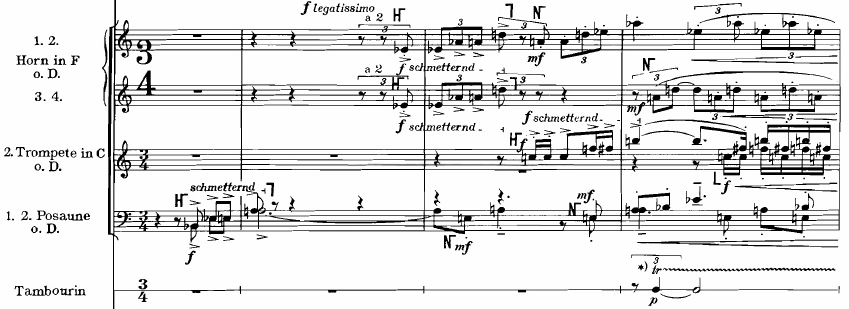
\includegraphics[width=\textwidth]{figures/berg2.png}
		\caption{Derived row in the \emph{Prologue} of Alban Berg's \emph{Lulu}.}
	\end{figure}
\end{frame}

%------------------------------------------------------------------------
\begin{frame}
	\frametitle{Derivation in Martino's \emph{Notturno}}
	\begin{block}{Example}
		Generate syntax from derivation by following $S$ with $V$ itself, then deriving a new row from $V$, say $Q$, and eventually following $V$ with $Q$. Repeating this procedure \emph{ad libitum} may generate many contrasting harmonic regions. If the chain of derived rows picked always the same order numbers, then a potential for rhythmic and agogic coherence could also be explored.
	\end{block}
\end{frame}


%------------------------------------------------------------------------
\begin{frame}
	\frametitle{Starr (1984)}
	\begin{block}{Definition}
		A totally constrained set with no precedence contradictions is a twelve-tone row. A completely unconstrained set of twelve tones represents the \textbf{free aggregate}. A maximally constrained one is called the \textbf{simultaneous aggregate} (a twelve-tone cluster).
	\end{block}
	\begin{block}{Definition}
		Consider the set $U$ of all ordered pairs of pitch classes -- this set has cardinality $12^2 = 144$. An element of $U$ is called an \textbf{order constraint}, and a subset $C$ of $U$ is called a \textbf{pitch-class relation}.
	\end{block}
\end{frame}

%------------------------------------------------------------------------
\begin{frame}
	\frametitle{Starr (1984)}
	\begin{block}{Proposition}
		Define a relation $x \sim y$ on the power set of $U$ by the set inclusion of the element $\{ x, y \}$. Then $\sim$ is an order relation on the set of twelve tones.
	\end{block}
	\begin{block}{Definition}
		A \textbf{partial order} is one that is reflexive, transitive, and antisymmetric, while a \textbf{total order} (a row), is a partial order that satisfies trichotomy.
	\end{block}
\end{frame}

%------------------------------------------------------------------------
\begin{frame}
	\frametitle{Starr (1984)}
	\begin{block}{Example}
		The free aggregate is a minimal reflexive subset of $U$ that contains all twelve tones.
	\end{block}
	\begin{block}{Definition}
		\textbf{Pruning} is the operation that removes redundancies due to transitivity from a pitch-class relation. Pruning can be reversed by \textbf{extension} to the point of its transitive closure. We say $x$ and $y$ are \textbf{incomparable} in $C$ if the latter lacks any order constraint involving both $\{ x, y \}$. \textbf{Linearizing} means injecting some constraint, as long as there remains a partial order. The set of all rows that can be linearized from some partial order is called its \textbf{total order class}. One can \textbf{verticalize} a pitch-class relation by removing constraints, as long as there remains a partial order. We say a partial order \textbf{covers} another whenever the former is a verticalization of the latter.
	\end{block}
\end{frame}

%------------------------------------------------------------------------
\begin{frame}
	\frametitle{Starr (1984)}
	\begin{block}{Example}
		To guarantee that a verticalization will remain a partial order, we take its union with the free aggregate (reflexivity), then subject this union to an extension operation (transitivity).
	\end{block}
	\begin{block}{Theorem}
		\begin{itemize}
        	\item Covering is transitive.
        	\item A pitch-class relation is covered by its extension.
        	\item If a pitch-class relation covers another, then the extension of the former covers the extension of the latter.
    	\end{itemize}
	\end{block}
\end{frame}

%------------------------------------------------------------------------
\begin{frame}
	\frametitle{Starr (1984)}
	\begin{block}{Theorem}
		Let $A$ and $B$ be partial orders and denote by $\Toc(A)$ and $\Toc(B)$ their respective total order classes. Then $A \cap B$ is again a partial order and
    	\begin{equation*}
        	\Toc(A) \cap \Toc(B) = \Toc(\Ext(A \cup B)) \enspace,
    	\end{equation*}
    	where $\Ext$ is the extension operator. Moreover, if $A_i$ is a finite sequence of $n$ partial orders, then
    	\begin{equation*}
        	\bigcap_{i = 0}^{n} \Toc(A_i) = \Toc \left[ \Ext\left ( \bigcup_{i = 0}^{n} A_i \right) \right] \enspace.
    	\end{equation*}
	\end{block}
\end{frame}

%------------------------------------------------------------------------
\begin{frame}
	\frametitle{Starr (1984)}
	\begin{block}{Theorem}
		Let $C$ be a pitch-class relation and $\{ a, b \}$ an element of $U$ such that $\{ a, b \} \in C$.
    	\begin{itemize}
        	\item If $F$ is a pitch-class operation, then $\{ F(a), F(b) \} \in F(C)$ if and only if $\{ a, b \} \in C$. In particular, if $\R(C)$ is the retrograde of $C$, then $\{ a, b \} \in \R(C)$ if and only if $\{ b, a \} \in C$.
        	\item If $C$ is totally ordered, then $\R(C) = (S \setminus D) \cup F$, where $S$ is the simultaneous aggregate and $F$ is the free aggregate.
        	\item If $C_1$ covers $C_2$, then $F(C_1)$ covers $F(C_2)$.
        	\item If $C$ is $F\R$-invariant, then all cycles in $F$ have length two.
    	\end{itemize}
	\end{block}
\end{frame}


%------------------------------------------------------------------------
\begin{frame}
	\frametitle{Aggregate Realizations}
	\begin{block}{Definition}
		An \textbf{aggregate realization} is a particular type of partial order $C$ in which, for any pair of pitch classes $a, b$, if $a$ and $b$ are incomparable in $C$, then the set of pitch classes that precede $a$ in $C$ is equal to the set of pitch classes that precede $b$ in $C$, and also the set of pitch classes that follow $a$ in $C$ is equal to the set of pitch classes that follow $b$ in $C$.
	\end{block}
	\begin{block}{Example}
		\begin{itemize}
			\item Aggregate realizations arise naturally from a total order in the sense that they belong to the set of all partial orders that are covered by said total order
			\item Aggregate realizations lead to a classification of partial orders, as well as to many musical applications
			\item An interesting compositional application of aggregate realizations is that of projecting a total order as a middle-ground entity
		\end{itemize}
	\end{block}
\end{frame}

%------------------------------------------------------------------------
\begin{frame}
	\frametitle{Aggregate Realization in Webern's \emph{Variations} Op.~27}
	\begin{figure}
		\centering
		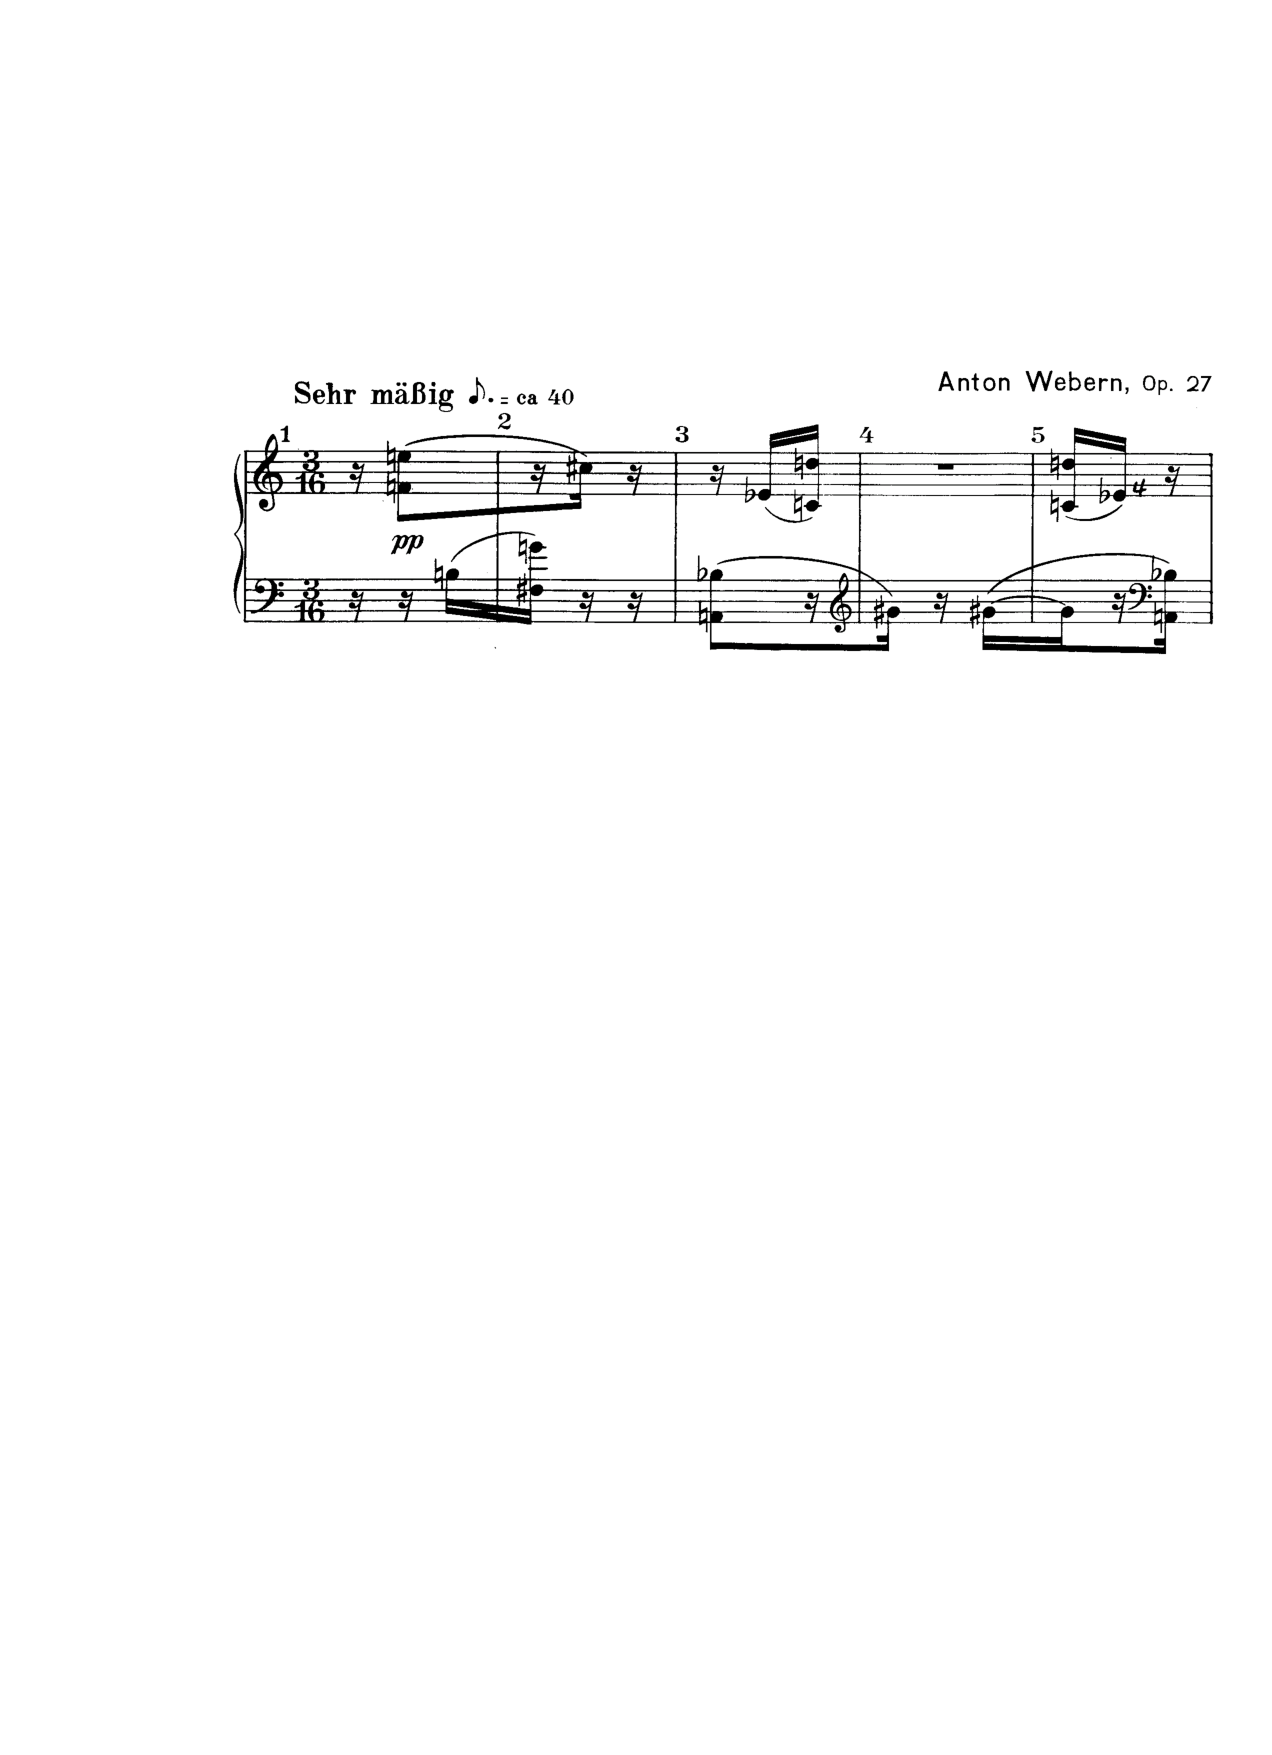
\includegraphics[width=\textwidth]{figures/webern1.pdf}
		\caption[Bars 1--7 in Webern's Op.~27]{The initial bars in Webern's Op.~27.}
	\end{figure}
\end{frame}

%------------------------------------------------------------------------
\begin{frame}[fragile]
	\frametitle{Aggregate Realization in Webern's \emph{Variations} Op.~27}
	\begin{figure}
		\centering
		\begin{adjustbox}{width=\textwidth}
		\begin{tikzcd}
			& E \arrow[dr] && G \arrow[dr] && B\flat \arrow[dr] && D \arrow[dr] & \\
			* \arrow[dr] \arrow[ur] && B \arrow[dr] \arrow[ur] && C\sharp \arrow[dr] \arrow[ur] && E\flat \arrow[dr] \arrow[ur] && G\sharp \\
			& F \arrow[ur] && F\sharp \arrow[ur] && A \arrow[ur] && C \arrow[ur] &
		\end{tikzcd}
		\end{adjustbox}
		\caption{An aggregate realization of the initial bars in Webern's Op.~27. At its very first presentation, the total order used to generate the piece cannot be discerned. Moreover, the partial order we are actually able to hear intercalates the total order's two hexachords, a procedure that can be construed as a form of derivation.}
	\end{figure}
\end{frame}

%------------------------------------------------------------------------
\begin{frame}
	\frametitle{Columnar Realizations}
	\begin{block}{Definition}
		A \textbf{columnar realization} is a set of disjoint row segments where the internal order of each segment is total, but all segments remain pairwise incomparable. We require that a columnar realization contain the free aggregate as a subset, so that we get all pitch classes belonging to a given base at each column.
	\end{block}
	\begin{block}{Example}
		\begin{itemize}
			\item The intersection of the set of all aggregate realizations with the set of all columnar realizations contains the set of all total orders, as well as the free aggregate.
			\item A total order is trivially an aggregate realization, and it is trivially a columnar realization; any total order contains the free aggregate per our requirements.
		\end{itemize}
	\end{block}
\end{frame}

%------------------------------------------------------------------------
\begin{frame}
	\frametitle{Row Segments}
	\begin{block}{Definition}
		A \textbf{row segment} is a pitch-class relation that is reflexive, transitive, and antisymmetric, where some subset of its order constraints also satisfy trichotomy. For any partial order that covers some row segment, we say that segment is an \textbf{embedded segment} of the partial order.
	\end{block}
	\begin{block}{Example}
		By transitivity of covering, any other partial order covering another will have the latter's row segments embedded in it. A partial order may be seen as the union (possibly the extension) of its various embedded segments.
	\end{block}
\end{frame}

%------------------------------------------------------------------------
\begin{frame}
	\frametitle{Row Segments}
	\begin{block}{Example}
		Let $X$ be an $n$-tone column vector, and consider the $n \times n$ matrix $A = [X, \cdots, X]$. The matrix $B = A - A^T$ will have a main diagonal of zeros, which indicates that $X$ shares with itself $n$ common tones under $T_0$. To find common tones under inversion, we let $B = A + A^T$ and, similarly, $\M$ and $\M \circ \I$ become $B = A - \M(A)^T$ and $B = A + \M(A)^T$. If the indices we are counting are disposed in any of the matrix's diagonals, then they will preserve ordering after the transform, thus becoming embedded segments; if, in addition, they are adjacent, then they will in fact be row segments shared by $X$ and its transform.
	\end{block}
\end{frame}

%------------------------------------------------------------------------
\begin{frame}
	\frametitle{Row Segments}
	\begin{block}{Example}
		If $n = 3$, then we have
		\begin{equation*}
			\T_3\I = (0 \; 3) (1 \; 2) (4 \; 11) (5 \; 10) (6 \; 9) (7 \; 8) \enspace.
		\end{equation*}
		Hence, under $\T_3\I$, every pitch-class in $S = \{ 0, 1, 4, 5, 8, 9 \}$ maps to the complement of $S$. If the operation is, for instance, $\T_9$, then since
		\begin{equation*}
			\T_9 = (0 \; 9 \; 6 \; 3) (1 \; 10 \; 7 \; 4) (2 \; 11 \; 8 \; 5) \enspace,
		\end{equation*}
		we get straightforwardly that $S = \{ 0, 1, 4, 5, 8, 9 \}$ shares three common tones with $\T_9(S)$, namely $0 \mapsto 9$, $4 \mapsto 1$, and $8 \mapsto 5$.
	\end{block}
\end{frame}

%------------------------------------------------------------------------
\begin{frame}
	\frametitle{Row Segments}
	\begin{block}{Definition}
		Let $X$ and $Y$ be row segments such that $X \cap Y = \emptyset$ as partial orders; the \textbf{concatenation} $X | Y$ is the partial order:
    	\begin{equation*}
        	X \cup Y \cup \{ \{ a, b \} : a \in X, b \in Y \} \enspace.
    	\end{equation*}
    	It follows both $X$ and $Y$ are embedded row segments of $X | Y$. Our use of concatenation is sequential -- the entire row segment $X$ precedes the entire row segment $Y$ in $X | Y$ -- thus we do not allow intercalation of segments when concatenating.
	\end{block}
\end{frame}


%------------------------------------------------------------------------
\begin{frame}
	\frametitle{Derivation with the Retrograde}
	\begin{table}
    	\caption{Schematics of a derivation procedure involving the retrograde and an arbitrary operation $F$.}
    	\centering
    	\vspace{12pt}
    	\begin{tabular}{c|cc}
        	\hline
        	& $S$ & $\R \circ F(S)$\\
        	\hline
        	$V$ & $V_1$ & $V_2$ \\
        	$\R \circ F(V)$ & $\R \circ F(V_2)$ & $\R \circ F(V_1)$ \\
        	\hline
    	\end{tabular}
	\end{table}
\end{frame}

%------------------------------------------------------------------------
\begin{frame}
	\frametitle{Derivation with the Retrograde}
	\begin{block}{Example}
		Take the row in Berg's \emph{Lulu}, $S = \{ 10, 2, 3, 0, 5, 7, 4, 6, 9, 8, 1, 11 \}$, and consider the segment $\vec{s} = [10 \; 0 \; 5 \; 7]^T$ as a column vector. Now let $A^T = [\;\vec{s} \; | \; \vec{s} \; | \; \vec{s} \; | \; \vec{s}\;]$ be the square matrix whose every column is equal to $\vec{s}$. Then
		\begin{equation*}
    		A + A^T = \begin{bmatrix}
    			2 & 10 & 3 & 5 \\
        		10 & 0 & 5 & 7 \\
        		3 & 5 & 10 & 0 \\
        		5 & 7 & 0 & 2
        	\end{bmatrix} \pmod{12} \enspace.
		\end{equation*}
		In particular, we see that the row segment $\{ 10, 0, 5, 7 \}$ is invariant under $\R\T_5\I$, since we get a main diagonal of fives when we mirror the matrix above vertically.
	\end{block}
\end{frame}

%------------------------------------------------------------------------
\begin{frame}
	\frametitle{Derivation with the Retrograde}
	\begin{block}{Example}
		If we match $S$ with $\R\T_5\I(S)$, we may get the row segment $\{ 10, 0, 5, 7 \}$ in the derived row $V$ itself, rather than in its retrograde. Setting it to $V_2$, say, yields $V = \{ 2, 3, 4, 6, 9, 8, 1, 11, 10, 0, 5, 7 \}$, so we get the combination matrix below.
		\begin{equation*}
    	\begin{adjustbox}{width=\textwidth}
    		$\left[\begin{array}{cccccccccccc|cccccccccccc}
        		. & 2 & 3 & . & . & . & 4 & 6 & 9 & 8 & 1 & 11 & . & . & . & . & . & . & 10 & 0 & 5 & . & . & 7 \\
        		10 & . & . & 0 & 5 & 7 & . & . & . & . & . & . & 6 & 4 & 9 & 8 & 11 & 1 & . & . & . & 2 & 3 & .
    		\end{array}\right]$
    	\end{adjustbox}
    	\end{equation*}
	\end{block}
\end{frame}

%------------------------------------------------------------------------
\begin{frame}
	\frametitle{Derivation with the Retrograde}
	\begin{block}{Proposition}
		Consider a 2-row combination matrix $C$ where a row is derived via the retrograde and some operation $F$. Denote the derived row by $V = V_1 | V_2$. Then the first column is the partial order $C_1 = V_1 \cup \R \circ \F(V_2)$, and similarly the second column is the partial order $C_2 = V_2 \cup \R \circ \F(V_1)$, such that $C_2 = \R \circ F(C_1)$. If $D$ is a partial order that covers $C_1$, then $\R \circ F(D)$ will cover $C_2$, and if $D$ is in the total order class of $C_1$, that is, $D$ is a row that can be linearized from $C_1$, then $\R \circ F(D)$ is in the total order class of $C_2$. Finally, 2-row derivations of this type exist for arbitrary rows. The number of such combination matrices for any given row depends on the invariances of the chosen partition of $V$.
	\end{block}
\end{frame}

%------------------------------------------------------------------------
\begin{frame}
	\frametitle{Folded Derivation}
	\begin{table}
    	\caption{Schematics of a folded derivation procedure involving the retrograde.}
    	\centering
    	\vspace{12pt}
    	\begin{tabular}{c|cc}
        	\hline
        	& $S$ & $\R \circ F(S)$\\
        	\hline
        	$V$ & $V_1$ & $V_2$ \\
        	$\R \circ F(V)$ & $\R \circ F(V_2)$ & $\R \circ F(V_1)$ \\
        	$\R \circ GF(V)$ & $\R \circ GF(V_2)$ & $\R \circ GF(V_1)$ \\
        	$G(V)$ & $G(V_1)$ & $G(V_2)$ \\
        	\hline
        	& $G(S)$ & $\R \circ GF(S) = \R \circ FG(S)$ \\
        	\hline
    	\end{tabular}
	\end{table}
\end{frame}

%------------------------------------------------------------------------
\begin{frame}
	\frametitle{Folded Derivation}
	\begin{block}{Example}
		Let $S = \{ 0, 1, 11, 3, 8, 10, 4, 9, 7, 6, 2, 5 \}$ and $V_1 = \{ 1, 3, 8, 9, 7, 2 \}$. Since the unordered set $V_1$ is $T_6$-invariant, we get $V_2 = \{ 11, 0, 10, 4, 5, 6 \}$ and the following combination matrix:
		\begin{equation*}
    	\begin{adjustbox}{width=\textwidth}
    		$\left[\begin{array}{cccccccccccc|cccccccccccc}
            	& 1 && 3 & 8 &&& 9 & 7 && 2 && 11 && 0 &&& 10 & 4 &&& 5 && 6 \\
            	0 && 11 &&& 10 & 4 &&& 6 && 5 && 8 && 1 & 3 &&& 2 & 9 && 7 &  
        	\end{array}\right]$
    	\end{adjustbox}
		\end{equation*}
		Since $S_1 = \{ 0, 1, 11, 3, 8, 10 \}$ maps to its complement under $\T_5\I$, we can use $S$ in a combination matrix where we match $S$ with its transform under $\T_5\I$ in the usual hexachordal combinatoriality way.
	\end{block}
\end{frame}

%------------------------------------------------------------------------
\begin{frame}
	\frametitle{Folded Derivation}
	\begin{block}{Example}
		We can then derive from $\T_5\I(S)$ the row $\T_5\I(V)$. Since $\T_5\I$ commutes with $T_6$, we get the following folded derivation:
		\begin{equation*}
    	\begin{adjustbox}{width=\textwidth}
        	$\left[\begin{array}{cccccccccccc|cccccccccccc}
            	& 1 && 3 & 8 &&& 9 & 7 && 2 && 11 && 0 &&& 10 & 4 &&& 5 && 6 \\
            	0 && 11 &&& 10 & 4 &&& 6 && 5 && 8 && 1 & 3 &&& 2 & 9 && 7 & \\
            	\hline
            	5 && 6 &&& 7 & 1 &&& 11 && 0 && 9 && 4 & 2 &&& 3 & 8 && 10 & \\
            	& 4 && 2 & 9 &&& 8 & 10 && 3 && 6 && 5 &&& 7 & 1 &&& 0 && 11
        	\end{array}\right]$
    	\end{adjustbox}
		\end{equation*}
	\end{block}
\end{frame}


%------------------------------------------------------------------------
\begin{frame}
	\frametitle{Shifted Derivation}
	\begin{table}
    	\caption{Schematics of a shifted derivation procedure involving the retrograde. The asterisk indicates there is no requirement we derive the same row class in both foldings, in which case $V$ would be replaced by some other row $V^*$ and $G$ could be the identity.}
    	\centering
    	\vspace{12pt}
    	\begin{tabular}{ c | c c c }
        	\hline%\noalign{\smallskip}
        	& $S$ & $\R \circ F(S)$ & \\
        	\hline
        	$V$ & $V_1$ & $V_2$ & \\
        	$\R \circ F(V)$ & $\R \circ F(V_2)$ & $\R \circ F(V_1)$ & \\
        	$\R \circ G(V)^*$ && $\R \circ G(V_2)^*$ & $\R \circ G(V_1)^*$ \\
        	$GF(V)^*$ && $GF(V_1)^*$ & $GF(V_2)^*$ \\
        	\hline
        	&& $GF(S)$ & $\R \circ G(S)$ \\
        	\hline
    	\end{tabular}
	\end{table}
\end{frame}

%------------------------------------------------------------------------
\begin{frame}
	\frametitle{Shifted Derivation}
	\begin{block}{Example}
		Consider the row $S = \{ 0, 1, 7, 2, 10, 9, 11, 4, 8, 5, 3, 6 \}$ and the combination matrix given by $\R\T_{10}\I(S)$ against $\T_{11}(S)$:
    	\begin{equation*}
        	\left[
        	\begin{array}{cccccccc|cccccccc}
            	4 && 7 && 5 && 2 && 6 & 11 & 1 & 0 & 8 & 3 & 9 & 10 \\
            	11 & 0 & 6 & 1 & 9 & 8 & 10 & 3 && 7 && 4 && 3 && 5
        	\end{array}
        	\right]
    	\end{equation*}
	\end{block}
\end{frame}

%------------------------------------------------------------------------
\begin{frame}
	\frametitle{Shifted Derivation}
	\begin{block}{Example}
		Deriving the row $V = V_1 | V_2 = \{ 1, 7, 2, 9, 8, 3 \} | \{ 4, 5, 6, 11, 0, 10 \}$ from $S | \R\T_{10}\I(S)$ yields the following shifted derivation:
		\begin{equation*}
    	\begin{adjustbox}{width=\textwidth}
        	$\left[
        	\begin{array}{cccccccccccc|cccccccc|c}
            	& 1 & 7 & 2 && 9 &&& 8 && 3 && 4 &&&& 5 &&&& 6 \\
            	0 &&&& 10 && 11 & 4 && 5 && 6 & && 7 &&&& 2 && \\
            	\hline
            	&&&&&&&&&&&& & 0 & 6 & 1 && 8 &&& 7 \\
            	&&&&&&&&&&&& 11 &&&& 9 && 10 & 3 &
        	\end{array}
        	\right. \cdots$
    	\end{adjustbox}
    	\end{equation*}
    	\begin{equation*}
    	\begin{adjustbox}{width=\textwidth}
        	$\cdots \left. \begin{array}{c|cccccccc|cccccccccccc}
            	& 6 & 11 && 0 &&&& 10 &&&&&&&&&&& \\
            	& && 1 && 8 & 3 & 9 & &&&&&&&&&&& \\
            	\hline
            	& 7 &&&& 3 &&& & 3 && 4 && 5 & 10 && 11 &&&& 9 \\
            	3 &&& 4 &&&& 5 & && 6 && 1 &&& 0 && 7 & 2 & 8
        	\end{array} \right]$
    	\end{adjustbox}
    	\end{equation*}
	\end{block}
\end{frame}

%------------------------------------------------------------------------
\begin{frame}
	\frametitle{Self Derivation}
	\begin{table}
    	\caption{Schematics of a self-derivation procedure involving the retrograde.}
    	\centering
    	\vspace{12pt}
    	\begin{tabular}{c|cc}
        	\hline
        	& $G(S)$ & $\R \circ FG(S)$ \\
        	\hline
        	$S$ & $S_1$ & $S_2$ \\
        	$\R \circ F(S)$ & $\R \circ F(S_2)$ & $\R \circ F(S_1)$ \\
        	\hline
    	\end{tabular}
	\end{table}
\end{frame}

%------------------------------------------------------------------------
\begin{frame}
	\frametitle{Self Derivation}
	\begin{block}{Example}
		Let $S = S_1 | S_2 = \{ 3, 8, 1, 0, 9, 6 \} | \{ 4, 7, 10, 5, 2, 11 \}$. In particular, both $S_1$ and $S_2$ are invariant under $\T_9\I$. What is not obvious is that we can derive $S$ and $\T_9\I(S)$ from a combination matrix where the first column is $\T_7(S)$ and the second is $\T_9\I \circ \R\T_7(S) = \R\T_2\I(S)$:
    	\begin{equation*}
    	\begin{adjustbox}{width=\textwidth}
        	$\left[
        	\begin{array}{cccccccccccc|cccccccccccc}
            	& 3 & 8 &&& 1 &&&& 0 & 9 & 6 &&&& 4 & 7 & 10 && 5 & 2 &&& 11 \\
            	10 &&& 7 & 4 && 11 & 2 & 5 &&&& 3 & 0 & 9 &&&& 8 &&& 1 & 6 &
        	\end{array}
        	\right]$
    	\end{adjustbox}
    	\end{equation*}
		Here we have $F = \T_9\I$ and $G = \T_7$. It is not the case that $F$ and $G$ commute, as $\T_2\I = F \circ G \ne G \circ F = \T_4\I$.
	\end{block}
\end{frame}

%------------------------------------------------------------------------
\begin{frame}
	\frametitle{Self Derivation}
	\begin{block}{Example}
		Let $S = \{ 0, 11, 5, 10, 4, 2, 7, 9, 8, 3, 6, 1 \}$ and consider the following combination matrix given by $T_2(S) | \R\T_2(S)$, whose derived rows are $S$ and $\R(S)$:
    	\begin{equation*}
    	\begin{adjustbox}{width=\textwidth}
        	$\left[
        	\begin{array}{cccccccccccc|cccccccccccc}
            	& 0 && 11 & 5 &&& 10 && 4 && 2 && 7 && 9 && 8 & 3 &&& 6 && 1 \\
            	1 && 6 &&& 3 & 8 && 9 && 7 && 2 && 4 && 10 &&& 5 & 11 && 0 &
        	\end{array}
        	\right]$
    	\end{adjustbox}
    	\end{equation*}
		Subjecting the entire matrix to $T_1$ yields:
    	\begin{equation*}
    	\begin{adjustbox}{width=\textwidth}
        	$\left[
        	\begin{array}{cccccccccccc|cccccccccccc}
            	& 1 && 0 & 6 &&& 11 && 5 && 3 && 8 && 10 && 9 & 4 &&& 7 && 2 \\
            	2 && 7 &&& 4 & 9 && 10 && 8 && 3 && 5 && 11 &&& 6 & 0 && 1 &
        	\end{array}
        	\right]$
    	\end{adjustbox}
    	\end{equation*}
	\end{block}
\end{frame}

%------------------------------------------------------------------------
\begin{frame}
	\frametitle{Self Derivation}
	\begin{block}{Example}
		We can then pull an entire matrix from the first row of above:
    	\begin{equation*}
    	\begin{adjustbox}{width=\textwidth}
        	$\left[
        	\begin{array}{cccccccccccc|cccccccccccc|c}
            	&&& 0 &&&& 11 && 5 &&&&&& 10 &&& 4 &&&&& 2 & \\
            	& 1 &&& 6 &&&&&&& 3 && 8 &&&& 9 &&&& 7 &&& 2 \\
            	2 && 7 &&& 4 & 9 && 10 && 8 && 3 && 5 && 11 &&& 6 & 0 && 1 &&
        	\end{array}
        	\cdots \right.$
    	\end{adjustbox}
    	\end{equation*}
	\end{block}
\end{frame}


%------------------------------------------------------------------------
\begin{frame}
	\frametitle{Derivation in Scotto's \emph{Tetralogy}}
	Let $S = \{ 0, 4, 7, 3, 11, 2, 10, 1, 6, 8, 9, 5 \}$ and consider the self-derivation array below.
    \begin{figure}
    	\centering
    	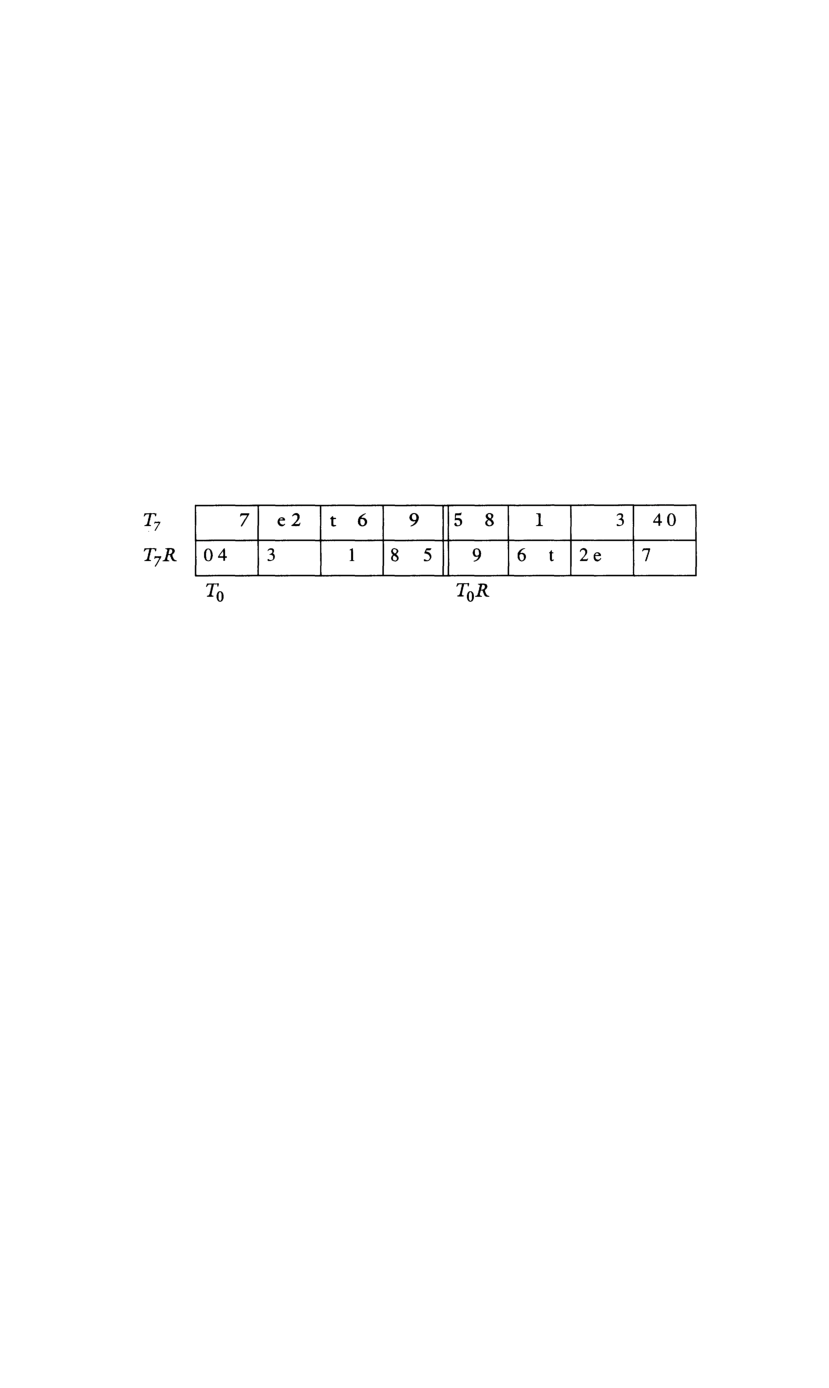
\includegraphics[width=\textwidth]{figures/scotto-array.pdf}
		\caption{Self-derived row in Scotto's \emph{Tetralogy}.}
	\end{figure}
\end{frame}

%------------------------------------------------------------------------
\begin{frame}
	\frametitle{Derivation in Scotto's \emph{Tetralogy}}
	We can fold the above matrix in order to obtain subsequent levels of derivation. The rows in the figure below are $\T_2(S), \R\T_2(S), \rho_6\R\T_2(S)$ and $\rho_6\T_2(S)$, where $\rho$ is the cyclical rotation operator.
	\begin{figure}
    	\centering
		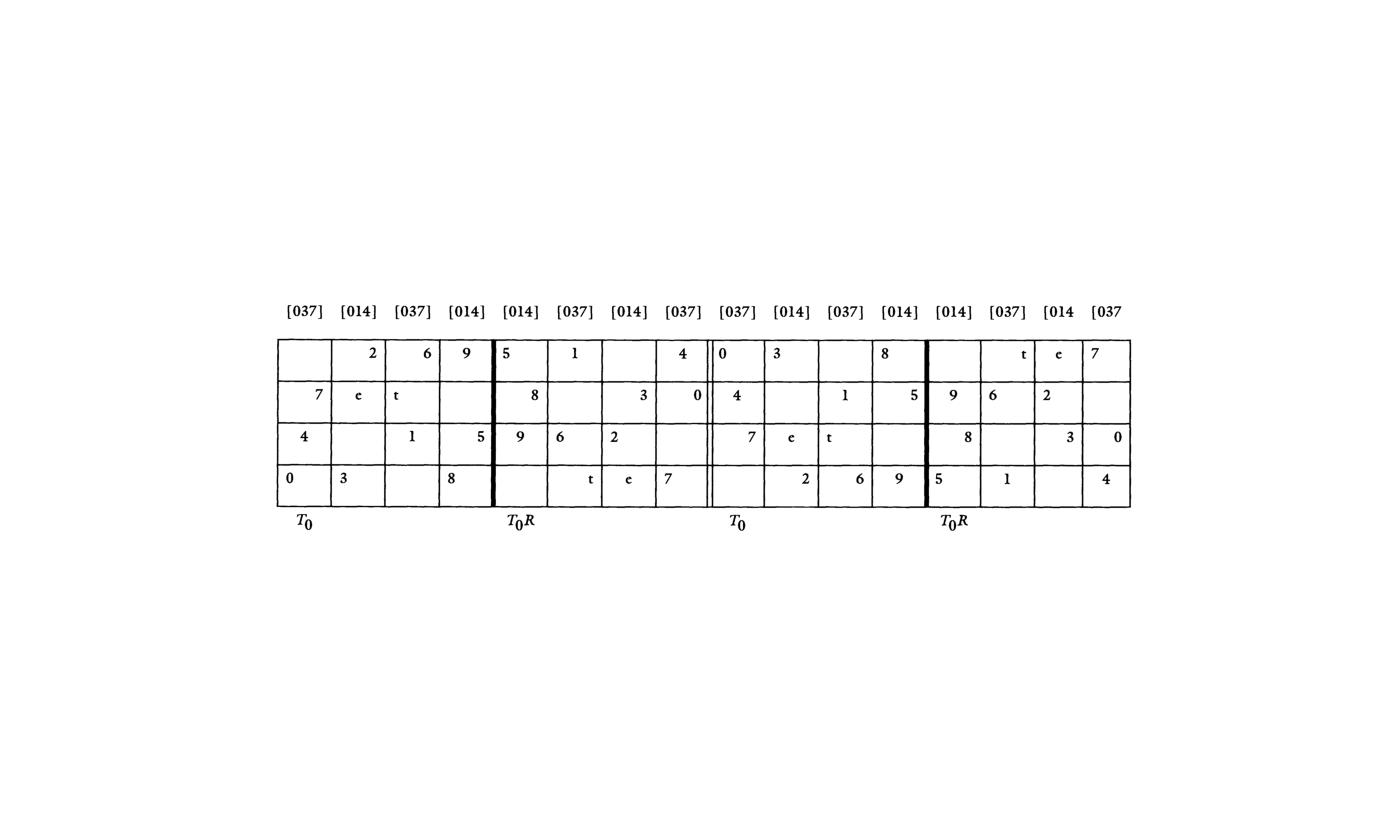
\includegraphics[width=3.2cm, angle=270]{figures/scotto-folded.pdf}
		\caption{Folded derivation in Scotto's \emph{Tetralogy}.}
	\end{figure}
\end{frame}

%------------------------------------------------------------------------
\begin{frame}
	\frametitle{Derivation in Scotto's \emph{Tetralogy}}
	\begin{figure}
    	\centering
		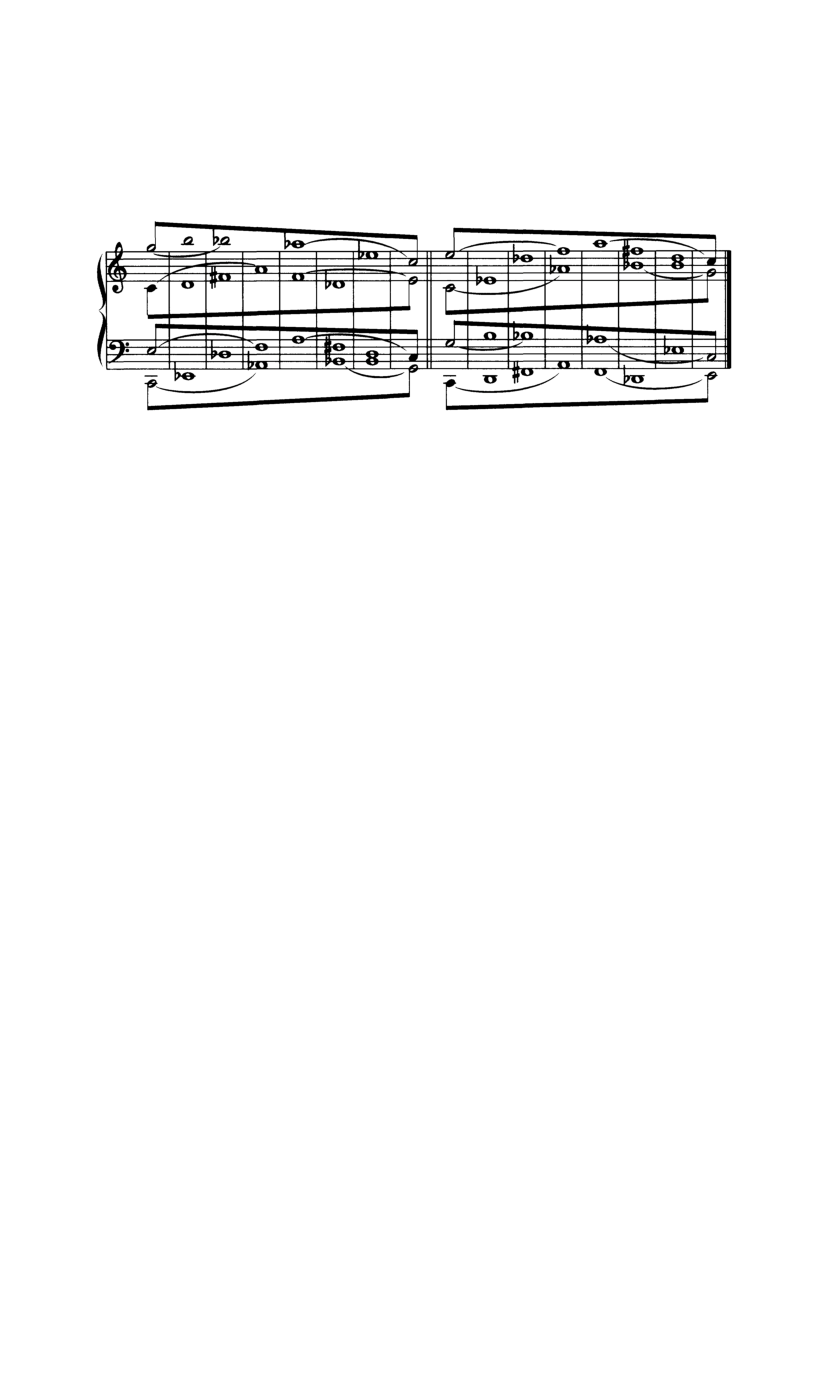
\includegraphics[width=\textwidth]{figures/scotto-schenker1.pdf}
		\caption{Schenkerian middle-ground structure in Scotto's \emph{Tetralogy}.}
	\end{figure}
\end{frame}

%------------------------------------------------------------------------
\begin{frame}
	\frametitle{Derivation in Scotto's \emph{Tetralogy}}
	\begin{figure}
    	\centering
    	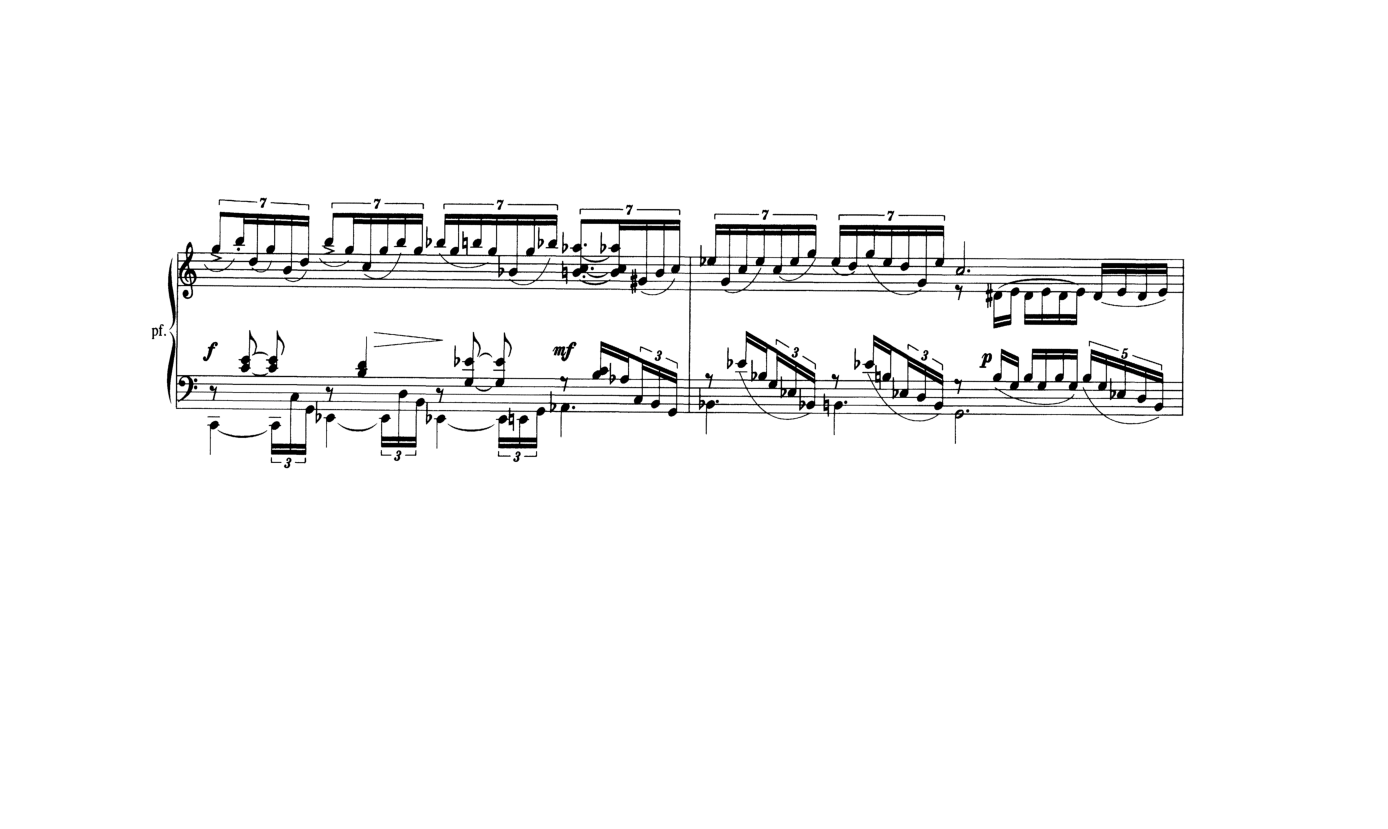
\includegraphics[width=3.2cm, angle=270]{figures/scotto-music1.pdf}
		\caption{Musical realization of the middle-ground in Scotto's \emph{Tetralogy}.}
	\end{figure}
\end{frame}

%------------------------------------------------------------------------
\begin{frame}
	\frametitle{Derivation in Scotto's \emph{Tetralogy}}
	The idea of prolongation in \emph{Tetralogy} extends beyond the foreground musical surface, and is applied as well to the middle-ground structure itself, effectively pushing it further into the background of the piece. 
	\begin{figure}
    	\centering
    	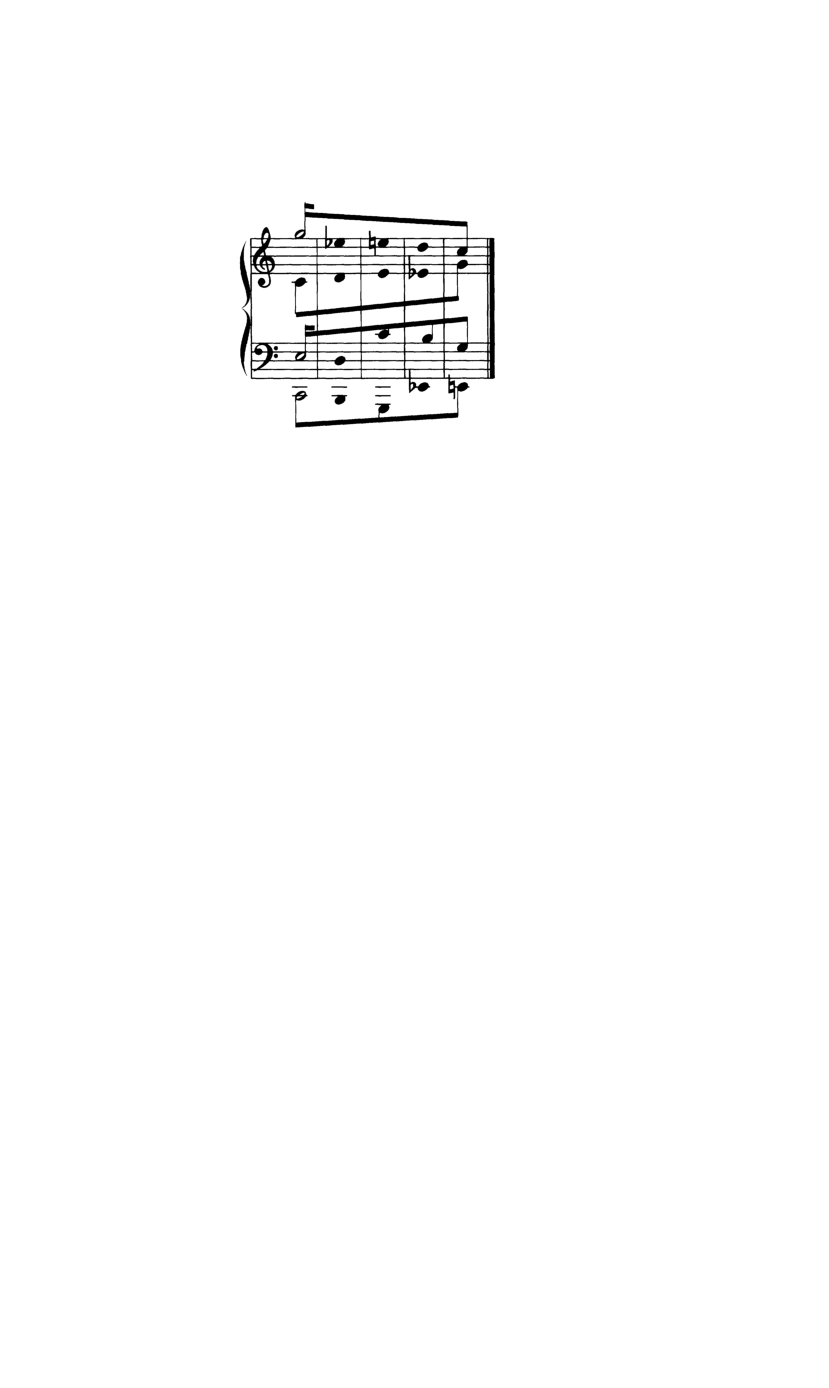
\includegraphics[width=5cm]{figures/scotto-schenker2.pdf}
    	\caption{Prolongation of the middle-ground structure in Scotto's \emph{Tetralogy}.}
	\end{figure}
\end{frame}

%------------------------------------------------------------------------
\begin{frame}
	\frametitle{Derivation in Scotto's \emph{Tetralogy}}
	\begin{figure}
    	\centering
    	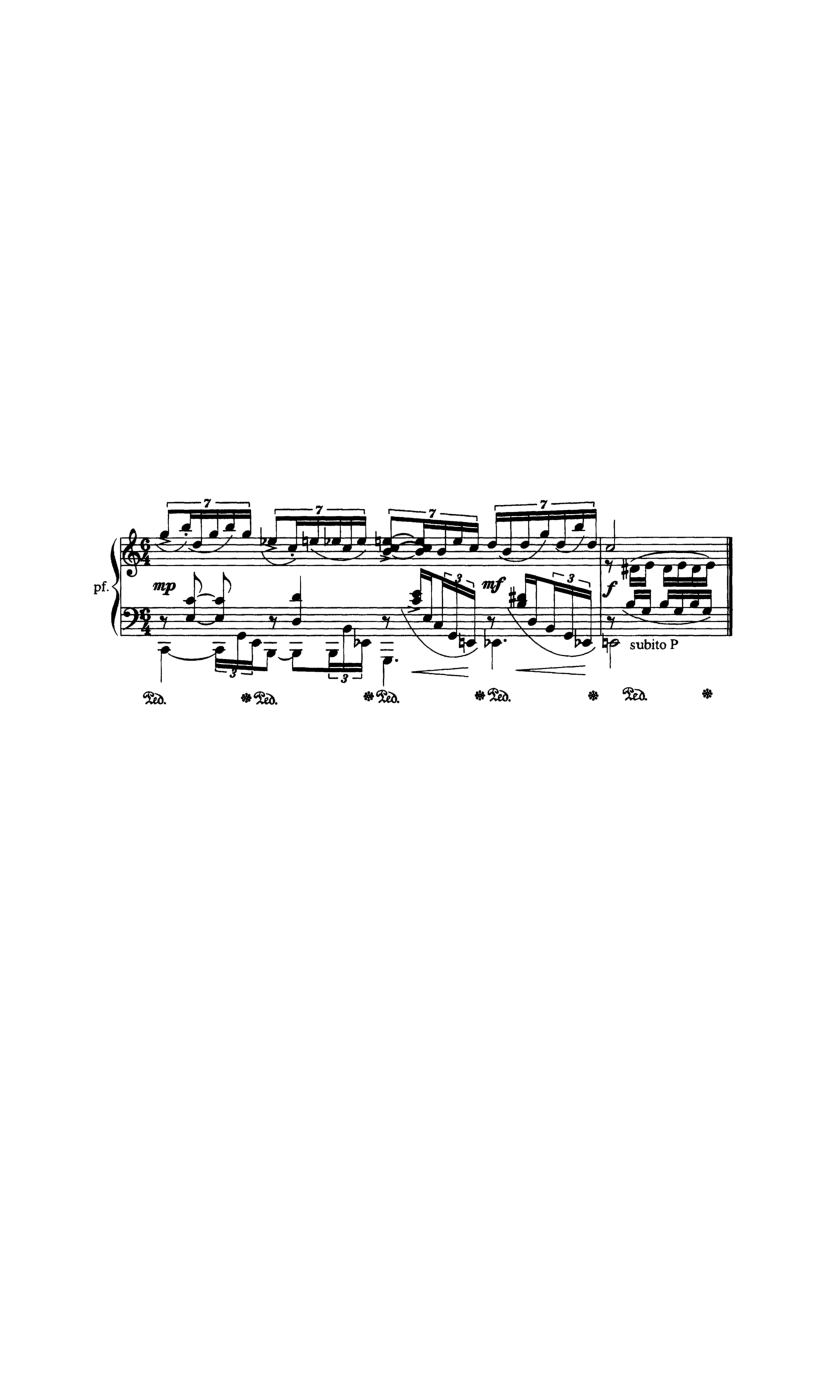
\includegraphics[width=\textwidth]{figures/scotto-music2.pdf}
    	\caption{Musical realization of the prolonged middle-ground in Scotto's \emph{Tetralogy}.}
	\end{figure}
\end{frame}


%------------------------------------------------------------------------
\begin{frame}
	\frametitle{Derivation from Aggregate Realizations}
	Let $S = \{ 0, 1, 7, 2 \} | \{ 10, 9 \} | \{ 11, 4, 8, 5 \} | \{ 3, 6 \}$ and consider the combination matrix below:
    \begin{equation*}
        A = \left[
        \begin{array}{c|c|c|c}
        	\{ 0, 1, 7, 2 \} & \{ 10, 9 \} & \{ 11, 4, 8, 5 \} & \{ 3, 6 \} \\
        	\{ 6, 3 \} & \{ 5, 8, 4, 11 \} & \{ 9, 10 \} & \{ 2, 7, 1, 0 \}
        \end{array}
        \right]
    \end{equation*}
	The first column of $A$ comprises the partial order $S_1 \cup \R(S_4)$, and this union maps onto its hexachordal complement under $\T_{11}\I$.
	\begin{equation*}
        \hat{A} = \left[
        \begin{array}{c|c|c|c}
        	\{ 0, 1, 7, 2 \} & \{ 10, 9 \} & \{ 11, 4, 8, 5 \} & \{ 3, 6 \} \\
        	\{ 6, 3 \} & \{ 5, 8, 4, 11 \} & \{ 9, 10 \} & \{ 2, 7, 1, 0 \} \\
        	\{ 11, 10, 4, 9 \} & \{ 1, 2 \} & \{ 0, 7, 3, 6 \} & \{ 8, 5 \} \\
        	\{ 5, 8 \} & \{ 6, 3, 7, 0 \} & \{ 2, 1 \} & \{ 9, 4, 10, 11 \}
        \end{array}
        \right]
    \end{equation*}
\end{frame}

%------------------------------------------------------------------------
\begin{frame}
	\frametitle{Derivation from Aggregate Realizations}
	Let $C_1, C_2, C_3, C_4$ be the four columns of the matrix $\hat{A}$. It follows the row $V = \{ 11, 0, 1, 6, 10, 4, 7, 2, 9, 5, 3, 8 \}$ has the property that $T \in \Toc \{ \Ext[ C_1 \cup \R\T_1\I(C_2) \cup \T_1\I(C_3) \cup \R(C_4) ] \}$. We can therefore derive $[V | \R\T_1\I(V) | \T_1\I(V) | \R(V)]$ from the columns of $\hat{A}$.
	\begin{equation*}
	\begin{adjustbox}{width=\textwidth}
        $\left[
        \begin{array}{cccccccccccc|cccccccccccc|c}
            & 0 & 1 &&&& 7 & 2 &&&& && 10 &&&&& 9 &&&&& & \\
            &&& 6 &&&&&&& 3 & & 5 && 8 & 4 & 11 &&&&&&& & \\
            \hline
            11 &&&& 10 & 4 &&& 9 &&& &&&&&&&&&&& 1 & 2 & \\
            &&&&&&&&& 5 && 8 &&&&&& 6 && 3 & 7 & 0 && & 2
        \end{array}
        \right. \cdots$
    \end{adjustbox}
    \end{equation*}
    \begin{equation*}
    \begin{adjustbox}{width=\textwidth}
        $\cdots \left.
        \begin{array}{c|cccccccccccc|cccccccccccc}
            & &&&&&&& 11 & 4 & 8 && 5 && 3 &&&&&&& 6 &&& \\
            & &&&&& 9 &&&&& 10 & &&&&& 2 & 7 &&&& 1 & 0 & \\
            \hline
            & && 0 & 7 & 3 && 6 &&&&& & 8 && 5 &&&&&&&&& \\
            2 & 2 & 1 &&&&&&&&&& &&&& 9 &&& 4 & 10 &&&& 11
        \end{array} \right]$
    \end{adjustbox}
    \end{equation*}
\end{frame}

%------------------------------------------------------------------------
\begin{frame}[fragile]
	\frametitle{Derivation from Aggregate Realizations}
	Let $S = \{ 0, 1, 7, 2 \} | \{ 10, 9, 11, 4 \} | \{ 8, 5, 3, 6 \} = S_1 | S_2 | S_3$ and consider the matrix $A = [S | \T_4(S) | \T_8(S)]^T$.
    \begin{equation*}
        A = \left[
        \begin{array}{cccc|cccc|cccc}
        	0 & 1 & 7 & 2 & 10 & 9 & 11 & 4 & 8 & 5 & 3 & 6 \\
        	4 & 5 & 11 & 6 & 2 & 1 & 3 & 8 & 0 & 9 & 7 & 10 \\
        	8 & 9 & 3 & 10 & 6 & 5 & 7 & 0 & 4 & 1 & 11 & 2
        \end{array}
        \right] \enspace.
    \end{equation*}
    Now let $V$ be in the total order class of the first columnar aggregate of $A$. Next, rewrite the first columnar aggregate of $A$ as the aggregate realization $A_1$.
    \begin{equation*}
    \begin{adjustbox}{width=\textwidth}
        $A_1 = \begin{tikzcd}
            & 0 \arrow[dr] && 1 \arrow[dr] && 7 \arrow[dr] && 2 \arrow[dr] & \\
            * \arrow[r] \arrow[dr] \arrow[ur] & 4 \arrow[r] & * \arrow[r] \arrow[dr] \arrow[ur] & 5 \arrow[r] & * \arrow[r] \arrow[dr] \arrow[ur] & 11 \arrow[r] & * \arrow[r] \arrow[dr] \arrow[ur] & 6 \arrow[r] & * \\
            & 8 \arrow[ur] && 9 \arrow[ur] && 3 \arrow[ur] && 10 \arrow[ur] &
        \end{tikzcd}$
    \end{adjustbox}
    \end{equation*}
\end{frame}

%------------------------------------------------------------------------
\begin{frame}
	\frametitle{Derivation from Aggregate Realizations}
	Any $V \in \Toc(A_1)$ must be a succession of augmented triads, say, $V = \{ 4, 8, 0, 9, 1, 5, 11, 7, 3, 2, 10, 6 \}$. We would like to linearize some transform of $V$ from the other columns of $A$. To verify that $A_2$ is a transform of $A_1$, check whether there is a base-four $\R\T_n\M\I$ operation that maps $S_1 \pmod 4$ onto $S_2 \pmod 4$.
    \begin{equation*}
        S_1 \pmod 4 = \{ 0, 1, 3, 2 \} = \T_2\I(\{ 2, 1, 3, 0 \}) = \T_2\I \circ S_2 \pmod 4 \enspace.
    \end{equation*}
    The elements in each of $A_1$'s columns are incomparable, so we pick from each column in any order we want. We can reduce all of $A$'s columns $\mod 4$ by construction, so it is enough to only consider each column's residue modulo four.
\end{frame}

%------------------------------------------------------------------------
\begin{frame}
	\frametitle{Derivation from Aggregate Realizations}
	Since $S_1 \pmod 4 = S_3 \pmod 4$, we can derive $V$ itself from $A_3$, and thus obtain the following derivation matrix, where the second column is $\T_2\I(V)$.
	    \begin{multline*}
        \left[
        \begin{array}{cccccccccccc|cccccc}
        	&& 0 && 1 &&& 7 && 2 && & 10 &&&&& 9 \\
        	4 &&&&& 5 & 11 &&&&& 6 & && 2 && 1 & \\
        	& 8 && 9 &&&&& 3 && 10 & & & 6 && 5 &&
        \end{array}
        \right. \cdots \\\\
        \cdots \left.
        \begin{array}{cccccc|cccccccccccc}
        	&& 11 && 4 & & & 8 &&&& 5 &&& 3 &&& 6 \\
        	3 &&&&& 8 & && 0 & 9 &&&& 7 &&& 10 & \\
        	& 7 && 0 && & 4 &&&& 1 && 11 &&& 2 &&
        \end{array}
        \right]
    \end{multline*}
\end{frame}

%------------------------------------------------------------------------
\begin{frame}[fragile]
	\frametitle{Derivation from Aggregate Realizations}
	Knowing that the columns of $A$ are related as aggregate realizations by the operation tuple $\mathcal{A} = [\T_0 \; \T_2\I \; \T_0]$, we can regard the $A_i$ as columnar aggregates, then take $\hat{A} = \Ext[\bigcup_i(\mathcal{A}_i \circ A_i)]$. Any row we are able to linearize from $\hat{A}$, will be in $\bigcap_i \Toc(A_i)$, and thus we can derive its $\mathcal{A}_i$-transform from each $i$-column of $A$.
	\begin{equation*}
        \hat{A} = \begin{tikzcd}
            & 0 \arrow[r] \arrow[ddr] & 1 \arrow[r] \arrow[dr] & 7 \arrow[r] \arrow[ddr] & 2 \arrow[dr] & \\
            * \arrow[r] \arrow[dr] \arrow[ur] & 4 \arrow[r] \arrow[ur] & 5 \arrow[r] \arrow[dr] & 11 \arrow[r] \arrow[ur] & 6 \arrow[r] & * \\
            & 8 \arrow[r] \arrow[ur] & 9 \arrow[r] \arrow[uur] & 3 \arrow[r] \arrow[ur] & 10 \arrow[ur] &
        \end{tikzcd}
    \end{equation*}
\end{frame}

%------------------------------------------------------------------------
\begin{frame}
	\frametitle{Derivation from Aggregate Realizations}
    It follows $\hat{V} = \{ 0, 1, 4, 8, 9, 5, 7, 2, 11, 3, 10, 6 \}$ can be linearized from $\hat{A}$.
    \begin{multline*}
        \left[
        \begin{array}{cccccccccccc|cccccc}
        	0 &&&& 1 & 7 &&& 2 &&&&&&& 10 && \\
        	&&& 4 &&& 5 & 11 &&& 6 && 2 &&&& 1 & \\
        	& 8 & 9 &&&&&&& 3 && 10 && 6 & 5 &&& 7
        \end{array}
        \right. \cdots \\\\
        \cdots \left.
        \begin{array}{cccccc|cccccccccccc}
        	9 &&& 11 && 4 && 8 &&&&& 5 &&& 3 & 6 & \\
        	& 3 &&& 8 && 0 && 9 &&& 7 &&&&&& 10 \\
        	&& 0 &&&&&&& 4 & 1 &&& 11 & 2 &&&
        \end{array}
        \right]
    \end{multline*}
\end{frame}


%------------------------------------------------------------------------
\begin{frame}[fragile]
	\frametitle{Derivation in Damiani's \emph{Stingray}}
	Consider the aggregate realization A.
	\begin{equation*}
	\begin{adjustbox}{height=3.2cm}
		$A = \begin{tikzcd}
			& 0 \arrow[dddr] && 1 \arrow[dddr] & \\
			& 4 \arrow[ddr] && 5 \arrow[ddr] & \\
			& 8 \arrow[dr] && 9 \arrow[dr] & \\
    		* \arrow[ur] \arrow[uur] \arrow[uuur] \arrow[dr] \arrow[ddr] \arrow[dddr] && * \arrow[ur] \arrow[uur] \arrow[uuur] \arrow[dr] \arrow[ddr] \arrow[dddr] && * \\
    		& 11 \arrow[ur] && 10 \arrow[ur] & \\
    		& 7 \arrow[uur] && 6 \arrow[uur] & \\
    		& 3 \arrow[uuur] && 2 \arrow[uuur] &
    	\end{tikzcd}$
    \end{adjustbox}
	\end{equation*}
\end{frame}

%------------------------------------------------------------------------
\begin{frame}
	\frametitle{Derivation in Damiani's \emph{Stingray}}
	$A$ is invariant under the set of operations $\Omega = \{ \T_0, \T_4, \T_8, \T_3\I, \T_7\I, \T_{11}\I \}$. Thus if $\rho \in \Toc(A)$, then also $\Omega_i(\rho) \in \Toc(A)$. Also, $\R(\rho) \in \Toc(\R \circ \Omega_i(A))$. Let $S = \{ 0, 1, 5, 8, 9, 4, 10, 3, 7, 6, 2, 11 \}$, and consider $\mathcal{A} = [\mathcal{A}_1 | \cdots | \mathcal{A}_6]$.
	\begin{equation*}
    	\mathcal{A} = \left[
    	\begin{array}{cc|cc|cc|cc|cc|cc}
    		0 & 1 & 5 & 8 & 9 & 4 & 10 & 3 & 7 & 6 & 2 & 11 \\
    		4 & 5 & 9 & 0 & 1 & 8 & 2 & 7 & 11 & 10 & 6 & 3 \\
    		8 & 9 & 1 & 4 & 5 & 0 & 6 & 11 & 3 & 2 & 10 & 7 \\
    		11 & 10 & 6 & 3 & 2 & 7 & 1 & 8 & 4 & 5 & 9 & 0 \\
    		7 & 6 & 2 & 11 & 10 & 3 & 9 & 4 & 0 & 1 & 5 & 8 \\
    		3 & 2 & 10 & 7 & 6 & 11 & 5 & 0 & 8 & 9 & 1 & 4
    	\end{array}
    	\right]
	\end{equation*}
\end{frame}

%------------------------------------------------------------------------
\begin{frame}
	\frametitle{Derivation in Damiani's \emph{Stingray}}
	Every row of $\mathcal{A}$ is an $\Omega$-transform of $S$. Every $\mathcal{A}_i$ is an instance of either $A$ or $\R(A)$, thus $\Omega$-invariant. We can derive a transform of $S$ from every $\mathcal{A}_i$. Since $\T_7(S) \in \Toc(\mathcal{A}_1)$ and $\R\T_0\I(S) \in \Toc(\mathcal{A}_2)$, we get $X$.
	\begin{equation*}
	\begin{adjustbox}{width=\textwidth}
    	$X = \left[
    	\begin{array}{cccccccccccc|cccccccccccc}
    		&&&&& 11 && 10 &&&&&&& 6 &&&&& 3 &&&& \\
    		&&&& 4 && 5 &&&&&&&&&& 9 &&&&&&& 0 \\
    		&&& 3 &&&&& 2 &&&&& 10 &&&&&&&& 7 && \\
    		&& 0 &&&&&&& 1 &&&&&& 5 &&& 8 &&&&& \\
    		& 8 &&&&&&&&& 9 && 1 &&&&&&&& 4 &&& \\
    		7 &&&&&&&&&&& 6 &&&&&& 2 &&&&& 11 &
    	\end{array}
    	\right]$
    \end{adjustbox}
	\end{equation*}
\end{frame}

%------------------------------------------------------------------------
\begin{frame}
	\frametitle{Derivation in Damiani's \emph{Stingray}}
	The transforms of $S$ we can derive from $\mathcal{A}_1$ and $\mathcal{A}_5$ are in
	\begin{equation*}
		\{ \T_3, \T_7, \T_{11}, \R\T_1, \R\T_5, \R\T_9, \T_0\I, \T_4\I, \T_8\I, \R\T_2\I, \R\T_6\I, \R\T_{10}\I \} \enspace.
	\end{equation*}
	For the columns $\mathcal{A}_2, \mathcal{A}_3, \mathcal{A}_4$ and $\mathcal{A}_6$, we can derive transforms of $S$ that are in
	\begin{equation*}
		\{ \T_1, \T_5, \T_9, \R\T_3, \R\T_7, \R\T_{11}, \T_2\I, \T_6\I, \T_{10}\I, \R\T_0\I, \R\T_4\I, \R\T_8\I \} \enspace.
	\end{equation*}
	One could take advantage of this fact by exploring contrasting harmonic regions.
\end{frame}

%------------------------------------------------------------------------
\begin{frame}
	\frametitle{Derivation in Damiani's \emph{Stingray}}
	\begin{figure}
    	\centering
		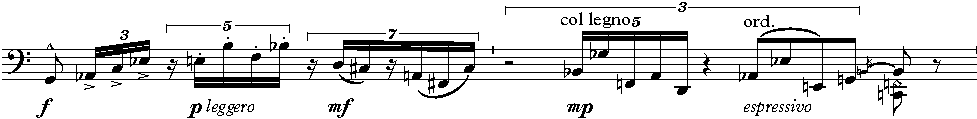
\includegraphics[width=\textwidth]{figures/stingray-example.pdf}
		\caption{Self-derivation in Damiani's \emph{Stingray}.}
	\end{figure}
\end{frame}


%------------------------------------------------------------------------
\begin{frame}
	\frametitle{The Mallalieu Property}
	\begin{block}{Example}
	Put $S^* = \{ 0, 1, 4, 2, 9, 5, 11, 3, 8, 10, 7, 6, * \}$. Then taking every zeroth order number of $S^* \mod 13$ yields trivially $S^*$ itself. Taking every first order number yields the row $\{ 1, 2, 5, 3, 10, 6, 0, 4, 9, 11, 8, 7, * \}$ which, upon removing the dummy symbol, becomes $\T_1(S)$. Repeating this procedure for every $n^\text{th}$ order number gives the sequence of $\T_i$-transforms of $S$ where the indices of transposition are totally-ordered, and correspond to the elements of $S$.
	\end{block}
\end{frame}

%------------------------------------------------------------------------
\begin{frame}
\frametitle{The Mallalieu Property}
	\begin{block}{Proposition}
		A 12-tone row has the mallalieu property if and only if it is related by $\T_n\M\I$ to the row $S = \{ 0, 1, 4, 2, 9, 5, 11, 3, 8, 10, 7, 6 \}$.
	\end{block}
	\begin{block}{Proof}
		One direction is just checking that every $\T_n\M\I$ transform of $S$ possesses the mallalieu property. Conversely, if a row $R$ in its untransposed prime form has the mallalieu property, then there is a transposition that takes its order numbers in zeroth rotation, that is, the set $\{ 0, 1, 2, 3, 4, 5, 6, 7, 8, 9, 10, 11 \}$ to its order numbers in, say, first rotation, id est, the set $\{ 1, 3, 5, 7, 9, 11, 0, 2, 4, 6, 8, 10 \}$. We can write this transposition as a permutation $0 \mapsto 1, 1 \mapsto 3, 2 \mapsto 5, \cdots, 11 \mapsto 10 $, or in cycle notation as $\hat{\T}_k = ( 0 \; 1 \; 3 \; 7 \; 2 \; 5 \; 11 \; 10 \; 8 \; 4 \; 9 \; 6 )$. Note that $\hat{\T}_k$ is an operation on order numbers.
	\end{block}
\end{frame}

%------------------------------------------------------------------------
\begin{frame}
\frametitle{The Mallalieu Property}
	\begin{block}{Proof}
	Since $\hat{\T}_k$ corresponds to a transposition, there are only four candidates for $T_k$, its pitch-class domain counterpart, namely $k \in \{ 1, 5, 7, 11 \}$, because these are the only indices for which a transposition of pitch classes in cycle notation is a 12-cycle. Moreover, we do not need to consider the cases where $k \in \{5, 7, 11\}$, as $\T_5 = \M \circ \T_1$, $\T_7 = \M \I \circ \T_1$, and $\T_{11} = \I \circ \T_1$. Hence, without loss, we can set $k = 1$. But then $S$ is the only row in untransposed prime form where $\T_1$ induces the permutation $\hat{\T}_k$ from its order numbers in zeroth rotation to its order numbers in first rotation. To see that, one needs to equate the cycles of $\hat{\T}_k$ with those of $\T_1$.
	\end{block}
\end{frame}

%------------------------------------------------------------------------
\begin{frame}
	\frametitle{The Mallalieu Property}
	\begin{block}{Example}
	Let $S = \{ 0, 1, 2, 3, 4, 5, 6, 7, 8, 9, 10, 11 \}$ and write $S^* = \{ 1, 2, 3, 4, 5, 6, 7, 8, 9, 10, 11, 12 \}$. Then $\M_3(S^*) = \{ 3, 6, 9, 12, 2, 5, 8, 11, 1, 4, 7, 10 \}$, which corresponds to the row $V = \{ 2, 5, 8, 11, 1, 4, 7, 10, 0, 3, 6, 9 \}$. The row $V$ can be constructed by placing an asterisk at the $13^\text{th}$ order number of $S$, then taking every third element. The fact that $V$ and $S$ are not related by $\T_n\M\I$ reflects the fact that neither $S$ nor $V$ have the mallalieu property.
	\end{block}
\end{frame}

%------------------------------------------------------------------------
\begin{frame}
	\frametitle{The Mallalieu Property}
	\begin{block}{Proposition}
	For $p$ a prime, every $(p - 1)$-TET system is capable of producing a mallalieu row.
	\end{block}
	\begin{block}{Example}
	The number of isomorphisms $\mathbb{Z} / 12 \mathbb{Z} \to (\mathbb{Z} / 13 \mathbb{Z})^\times$ is equal to
	\begin{equation*}
		|\Aut\big(\mathbb{Z} / 12 \mathbb{Z}\big)| = 4 \enspace.
	\end{equation*}
	If we map a generator of $\mathbb{Z} / 12 \mathbb{Z}$, say $\bar{1}$, to the generators of $(\mathbb{Z} / 13 \mathbb{Z})^\times$, namely $\bar{2}, \bar{6}, \bar{7}$ and $\overline{11}$, we obtain the four maps $i \pmod{12} \mapsto 2^i \pmod{13}$, $i \pmod{12} \mapsto 6^i \pmod{13}$, $i \pmod{12} \mapsto 7^i \pmod{13}$, and $i \pmod{12} \mapsto 11^i \pmod{13}$.
	\end{block}
\end{frame}

%------------------------------------------------------------------------
\begin{frame}
	\frametitle{The Mallalieu Property}
	\begin{block}{Example}
	Denote the first map by $\varphi$. Then
	\begin{equation*}
		\varphi(a + b) = 2^{a + b} = 2^a \cdot 2^b = \varphi(a) \cdot \varphi(b) \enspace,
	\end{equation*}
	so $\varphi$ is an isomorphism. Define $\varphi^{-1} : (\mathbb{Z} / 13 \mathbb{Z})^\times \to \mathbb{Z} / 12 \mathbb{Z}$ by
	$$\varphi^{-1}(\log i \pmod{13}) = i \pmod{12} \enspace.$$
	Let $S^* = \{ 1, 2, \dots, 11, 12 \}$ be a series of order numbers written multiplicatively. Then
	\begin{equation*}
		\varphi^{-1}(S^*) = \{ \log 1, \log 2, \dots, \log 12 \} \pmod{13} =
		\{ 0, 1, 4, \dots, 7, 6 \} \enspace.
	\end{equation*}
	\end{block}
\end{frame}


%------------------------------------------------------------------------
\begin{frame}
	\frametitle{Main Objectives}
	\begin{itemize}
		\item Study the application of self-derivation matrices to the algorithmic composition of acoustic and electroacoustic music
		\item Generalize the work of Starr (1984) to arbitrary equal-temperament systems
		\item Provide a solid mathematical foundation that describes the derivation of multiple order-number function arrays (required for non-brute-force algorithms)
		\item Confront findings with those of Kowalski (1987)
	\end{itemize}
\end{frame}

%------------------------------------------------------------------------
\begin{frame}
	\frametitle{Specific Questions}
	\begin{itemize}
		\item For any given row, determine whether it is capable of producing any known form of self-derivation
		\item Conversely, given some self-derivation procedure, provide a complete description of the class of rows that participate therein
		\item Extend the above to cases where the derived row is not in the same row class as the originating row
		\item Given a pattern of order numbers, understand what rows, and under which operations, yield known forms of derivation and self-derivation
		\item Investigate how chains of pitch-class operations are induced by derivation procedures and conversely
	\end{itemize}
\end{frame}

%------------------------------------------------------------------------
\begin{frame}
	\frametitle{Specific Questions}
	\begin{itemize}
		\item Make precise what the constraints regarding the choice of operation are for folded and shifted derivations
		\item Investigate the need for commutativity, and determine how the aforementioned forms support derivation without the retrograde
		\item Describe the role of the cyclic rotation operator, particularly in what regards folded self-derivations
		\item Generalize mallalieu rows to arbitrary equal temperament systems, giving a precise count and description of their untransposed representatives
		\item Investigate generalizations of the mallalieu property by relaxing the requirement that we get a copy of the row at \emph{every} index
		\item Describe mallalieu rows arising from operations other than transposition
	\end{itemize}
\end{frame}

%------------------------------------------------------------------------
\begin{frame}
	\frametitle{Expected Results}
	\begin{itemize}
		\item Provide a complete classification of rows that support self-derivation in matrices of all sizes
		\item Classify the algebraic operations that afford self-derivation
		\item Create general-purpose and non-brute-force algorithms to implement findings in the programming languages that pertain to musicians the most
		\item Compose pieces that illustrating the real-life use of such algorithms
		\item Provide criticism as to where such compositional practices situate within 21\textsuperscript{st}-century music composition
	\end{itemize}
\end{frame}

%------------------------------------------------------------------------
\begin{frame}
	\frametitle{Chapter Outline}
	\begin{itemize}
		\item Introduction
		\item Literature Review
		\item Theoretical Framework
		\item Summary of Results
		\item Compositional Applications
	\end{itemize}
\end{frame}

%
%------------------------------------------------------------------------
\begin{frame}
\frametitle{Title}
\begin{example}
Some text.
\end{example}
\end{frame}

%------------------------------------------------------------------------
\begin{frame}[allowframebreaks]
\frametitle{References}
\footnotesize{\begin{thebibliography}{1}
\bibitem{scotto} Scotto, C.: A Hybrid Compositional System: Pitch-Class Composition with Tonal Syntax. Perspectives of New Music 38(1), 169--222 (2000)
\end{thebibliography}}
\end{frame}


\end{document}
